\section{UI/UX Design \& High-Fidelity Mockups}
\label{sec:uiux}

\subsection{Core Design Philosophy: ``Less is More, Content-First''}
\label{subsec:ui_philosophy}

The user interface of \textbf{Naomi} is governed by a strict \textbf{Content-First Minimalist Philosophy} combining \textbf{Material Design 3} and \textbf{Apple Human Interface Guidelines (HIG)} across six non-negotiable design rules:
\begin{enumerate}
    \item \textbf{Elimination of Visual Clutter:} Zero marketing slogans, zero mood-tag bloat, and zero promotional banners; every screen displays only the exact controls and artwork required for the task.
    \item \textbf{Icon-Only Reader Toolbar:} All action controls on the \texttt{S05} Reader top bar use intuitive iconography without text labels to maximise unobstructed manga artwork area ($100\%$ viewport canvas).
    \item \textbf{Muted Minimal Color Palette:} Avoids neon gradients or multi-hue noise; uses calm monochrome neutrals paired with a single soft smoky-lavender accent (\texttt{\#7066A6}) so colorful comic covers and black-and-white manga ink take $100\%$ visual focus.
    \item \textbf{100\% International English UI Copy:} All labels, buttons, status indicators, and empty/error states use clean English microcopy (\textit{Sign In, Continue, Favorites, Offline Reading, Oops! No internet connection}).
    \item \textbf{100\% Authentic Manga Artwork:} All 12 frames render authentic MangaDex cover and page artwork (\textit{Frieren: Beyond Journey's End, Delicious in Dungeon, Yokohama Kaidashi Kikou, Witch Hat Atelier, The Apothecary Diaries, Mushishi}), never grey wireframe boxes.
    \item \textbf{Full-Chapter Pre-Buffering (\texttt{S10}):} Preloads $100\%$ of chapter pages prior to opening \texttt{S05} to guarantee zero mid-chapter loading spinners.
\end{enumerate}

\noindent\textbf{Interactive Prototype \& Figma Artifacts:}
\begin{itemize}
    \item \textbf{Figma Design File ($390 \times 844\text{ px}$ viewport):} \url{https://www.figma.com/design/flQOgQxYD3xWOUEpsnAUlM?node-id=1-3}
    \item \textbf{Local Interactive HTML5/JS Prototype:} Included in the repository at \texttt{document/naomi-ui-prototype/index.html} (supporting live frame switching across all 12 screens).
\end{itemize}

\subsection{Minimal Design Tokens \& Accessibility Standards}
\label{subsec:design_tokens}

Table~\ref{tab:design_tokens} defines the complete colour, typography, and spatial token system of \textbf{Naomi}, engineered to exceed \textbf{WCAG 2.1 AA/AAA} contrast ratios ($13.5\text{:}1$ on light surfaces; $14.2\text{:}1$ on dark reader surfaces) and $\ge 48 \times 48\text{ dp}$ touch target ergonomics (\texttt{NFR-15}).

\begin{table}[H]
\centering
\caption{Minimalist Muted Soft Palette, Spatial Grid, and Accessibility Tokens.}
\label{tab:design_tokens}
\footnotesize
\renewcommand{\arraystretch}{1.22}
\begin{tabularx}{\textwidth}{L{3.2cm} C{2.3cm} C{1.8cm} Y}
\toprule
\rowcolor{tablehead}
\textbf{Token Name} & \textbf{Hex / Value} & \textbf{Swatch} & \textbf{Semantic Usage \& Accessibility Role} \\
\midrule
\texttt{bg/canvas} & \texttt{\#F8F8FC} & \fcolorbox{gray}{naomicanvas}{\rule{0pt}{6pt}\rule{14pt}{0pt}} & Soft off-white primary background preventing eye glare during daytime browsing (\texttt{S01--S04, S07--S09, S11}). \\
\rowcolor{tablerow}
\texttt{bg/surface} \& \texttt{subtle} & \texttt{\#FFFFFF} / \texttt{\#EFEFF4} & \fcolorbox{gray}{white}{\rule{0pt}{6pt}\rule{14pt}{0pt}} & Elevated card containers, input fields, and subtle dividers. \\
\texttt{text/primary} \& \texttt{secondary} & \texttt{\#1C1C26} / \texttt{\#757588} & \fcolorbox{gray}{naomidark}{\rule{0pt}{6pt}\rule{14pt}{0pt}} & Deep charcoal primary typography ($13.5\text{:}1$ contrast) and muted slate metadata text. \\
\rowcolor{tablerow}
\texttt{brand/accent} \& \texttt{tint} & \texttt{\#7066A6} / \texttt{\#F0EFF8} & \fcolorbox{gray}{naomiaccent}{\rule{0pt}{6pt}\rule{14pt}{0pt}} & \textbf{Single Soft Accent:} Smoky pastel lavender for primary CTAs, progress bars, and the \texttt{S02} Hero card tint. \\
\texttt{reader/bg} \& \texttt{surface} & \texttt{\#111116} / \texttt{rgba(22,22,28,.9)} & \fcolorbox{gray}{black!90}{\rule{0pt}{6pt}\rule{14pt}{0pt}} & True AMOLED dark reader backdrop (\texttt{S05, S06, S10}) saving up to $30\%$ OLED power (\texttt{NFR-16}). \\
\rowcolor{tablerow}
\texttt{semantic/fav, ok, off} & \texttt{\#E05353}\newline \texttt{\#34A853}\newline \texttt{\#D97706} & \fcolorbox{gray}{mustgreen}{\rule{0pt}{6pt}\rule{14pt}{0pt}} & Muted coral red (\textit{Favorite}), sage green (\textit{Saved / Download 68\%}), and soft amber (\textit{Offline Warning}). \\
\textbf{Grid, Radii \& Touch} & \texttt{8px} grid, \texttt{48dp} target & --- & Card radius \texttt{12px}; Library big buttons \texttt{20px}; Dialog/Toolbar \texttt{16px}; all icons inside $\ge 48 \times 48\text{ dp}$ hit boxes. \\
\bottomrule
\end{tabularx}
\end{table}

\subsection{Complete Screen Navigation \& User Flow Architecture}
\label{subsec:user_flow}

Figure~\ref{fig:screen_flow} maps the complete end-to-end navigation graph across all 12 screens (\texttt{S01} through \texttt{S11}, including \texttt{S03b}), covering normal reading flows, audio sheet overlays, chapter preloading, active download progress, and offline network loss recovery.

\begin{figure}[H]
\centering
\begin{tikzpicture}[
    scr/.style={draw=hcmutblue!80!black, rounded corners=3pt, fill=white, line width=0.65pt, minimum height=0.8cm, text width=3.1cm, align=center, font=\tiny\sffamily},
    darkscr/.style={draw=naomiaccent!90!black, rounded corners=3pt, fill=naomitint, line width=0.75pt, minimum height=0.8cm, text width=3.1cm, align=center, font=\tiny\sffamily},
    errscr/.style={draw=couldamber!90!black, rounded corners=3pt, fill=orange!8, line width=0.75pt, minimum height=0.8cm, text width=3.1cm, align=center, font=\tiny\sffamily},
    arr/.style={-{Stealth[length=1.8mm,width=1.3mm]}, line width=0.65pt, draw=naomidark},
    darr/.style={-{Stealth[length=1.8mm,width=1.3mm]}, line width=0.65pt, dashed, draw=couldamber!90!black},
    lbl/.style={font=\tiny\sffamily, inner sep=1pt, fill=white}
]
    \node[scr] (s01) at (0,0) {\textbf{S01: Sign In}\\Email + Password | Sign Up};
    \node[scr] (s02) at (4.2,0) {\textbf{S02: Home}\\Hero Continue $\cdot$ Recent $\cdot$ Rec};
    \node[scr] (s03) at (8.4,0) {\textbf{S03: Discover}\\Search + AI Photo $\cdot$ Trending};
    \node[scr] (s03b) at (12.6,0) {\textbf{S03b: Expanded List}\\Full 2-Col Paginated Grid};

    \node[scr] (s08) at (0,-1.8) {\textbf{S08: Profile \& Settings}\\Theme $\cdot$ Lang $\cdot$ Cache $\cdot$ Out};
    \node[scr] (s07) at (4.2,-1.8) {\textbf{S07: Library (2 Big Btns)}\\1. Favorites \quad 2. Offline};
    \node[scr] (s04) at (8.4,-1.8) {\textbf{S04: Manga Detail}\\4 Action Btns + Chapter List};
    \node[errscr] (s11) at (12.6,-1.8) {\textbf{S11: Download Progress}\\68\% Bar + Bottom Toast};

    \node[errscr] (s09) at (4.2,-3.6) {\textbf{S09: Offline Error State}\\Oops! No Internet $\to$ CTA};
    \node[darkscr] (s10) at (8.4,-3.6) {\textbf{S10: Full Chapter Preload}\\42/42 Pages Ready (100\%)};
    \node[darkscr] (s05) at (12.6,-3.6) {\textbf{S05: Full Screen Reader}\\100\% Artwork + Top Icon Bar};
    \node[darkscr] (s06) at (12.6,-5.1) {\textbf{S06: Audio Sheet}\\Genre Instrumental Controls};

    \draw[arr] (s01) -- node[above, lbl]{Auth OK} (s02);
    \draw[arr, <->] (s02) -- node[above, lbl]{Bottom Nav} (s03);
    \draw[arr] (s03) -- node[above, lbl]{Tap [>]} (s03b);
    \draw[arr] (s03b) -- (s04);
    \draw[arr] (s03) -- (s04);
    \draw[arr] (s02) -- (s04);
    \draw[arr, <->] (s02) -- (s07);
    \draw[arr, <->] (s02) -- (s08);
    \draw[arr] (s02.south east) -- node[pos=0.4, lbl]{Continue} (s10.north west);
    \draw[arr] (s04) -- node[right, lbl]{Read Ch.} (s10);
    \draw[arr] (s10) -- node[above, lbl]{100\% Ready} (s05);
    \draw[arr, <->] (s05) -- node[right, lbl]{Tap $\flat$} (s06);
    \draw[arr] (s04) -- node[above, lbl]{Download} (s11);
    \draw[arr] (s11.south west) -- ++(-2.5,-0.55) -| node[pos=0.3, above, lbl]{Saved} (s07.south east);
    \draw[darr] (s04) -- node[above, sloped, lbl]{No Net (Uncached)} (s09);
    \draw[arr] (s09) -- node[right, lbl]{Go to Offline} (s07);
\end{tikzpicture}
\caption{Complete User Flow and Screen Navigation Graph across all 12 frames (\texttt{S01} to \texttt{S11}).}
\label{fig:screen_flow}
\end{figure}

\subsection{High-Fidelity Mobile Mockups \& Screen-by-Screen Specifications}
\label{subsec:hi_fi_mockups}

Figures~\ref{fig:mockups_group1}, \ref{fig:mockups_group2}, and \ref{fig:mockups_group3} present the 12 high-fidelity $390 \times 844\text{ px}$ mobile mockups rendered directly from the \textbf{Naomi} design system, followed by Table~\ref{tab:screen_catalog} detailing the functional components and state coverage of every frame.

\begin{figure}[H]
    \centering
    \begin{subfigure}[b]{0.24\textwidth}
        \centering
        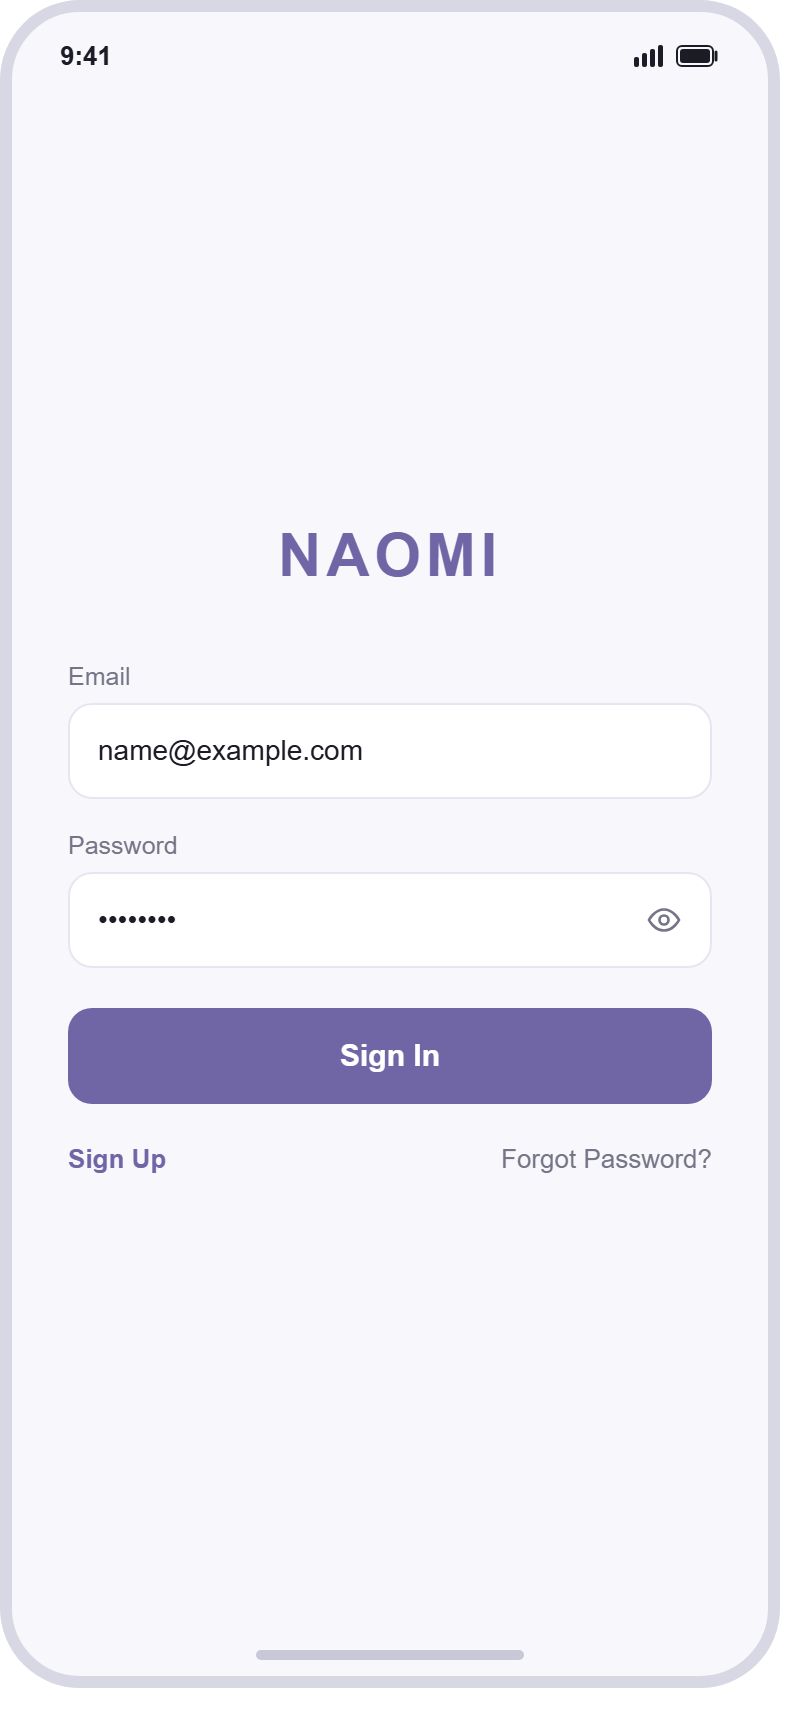
\includegraphics[width=\textwidth]{figures/ui/S01.png}
        \caption{\textbf{S01:} Sign In}
    \end{subfigure}
    \hfill
    \begin{subfigure}[b]{0.24\textwidth}
        \centering
        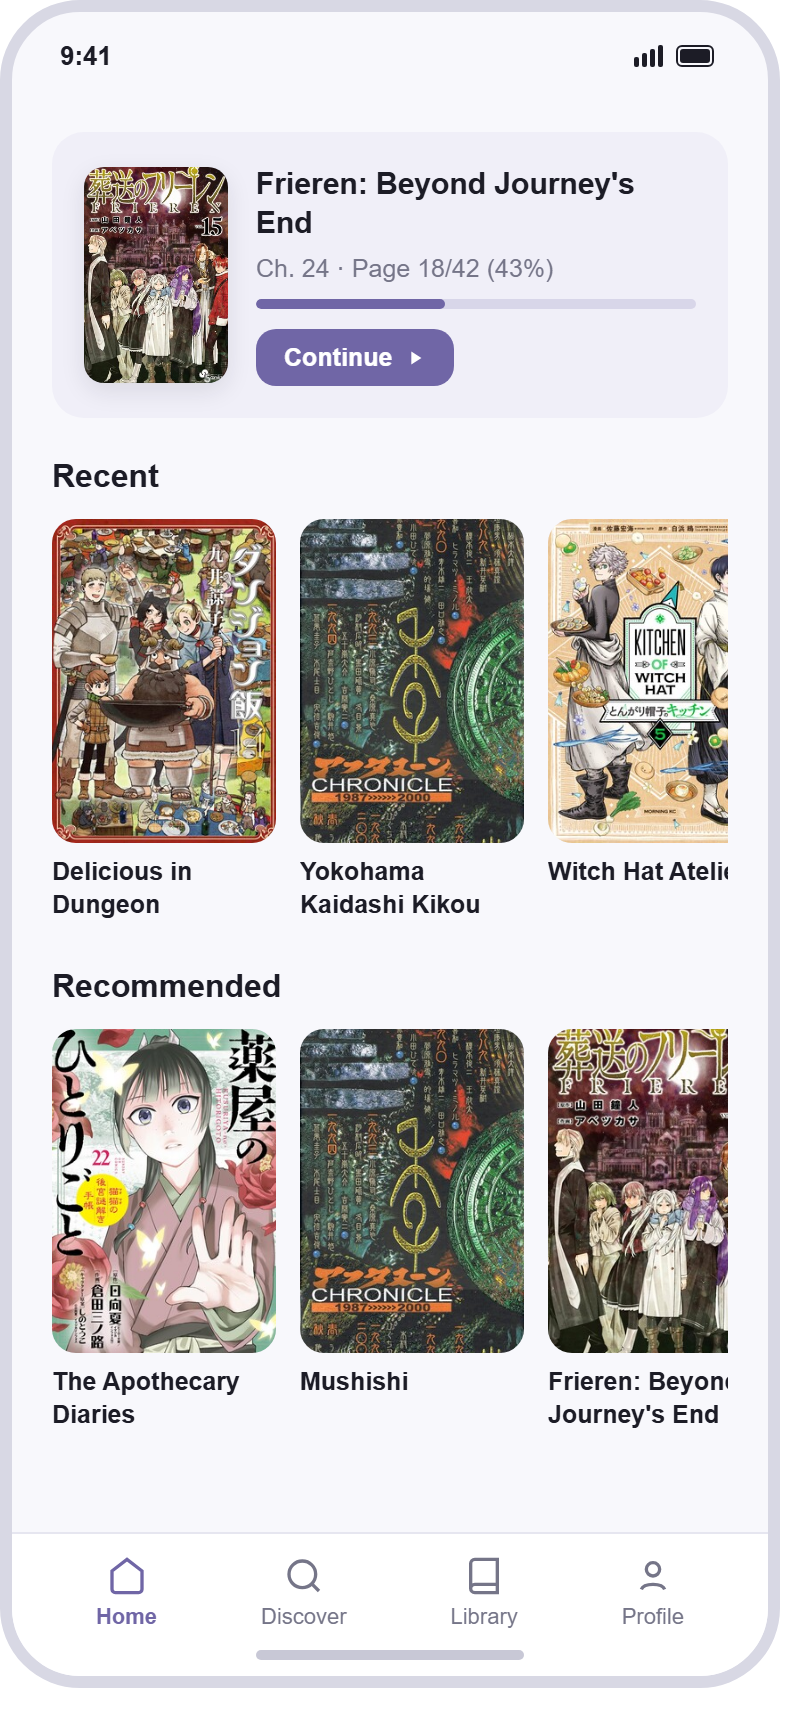
\includegraphics[width=\textwidth]{figures/ui/S02.png}
        \caption{\textbf{S02:} Home Feed}
    \end{subfigure}
    \hfill
    \begin{subfigure}[b]{0.24\textwidth}
        \centering
        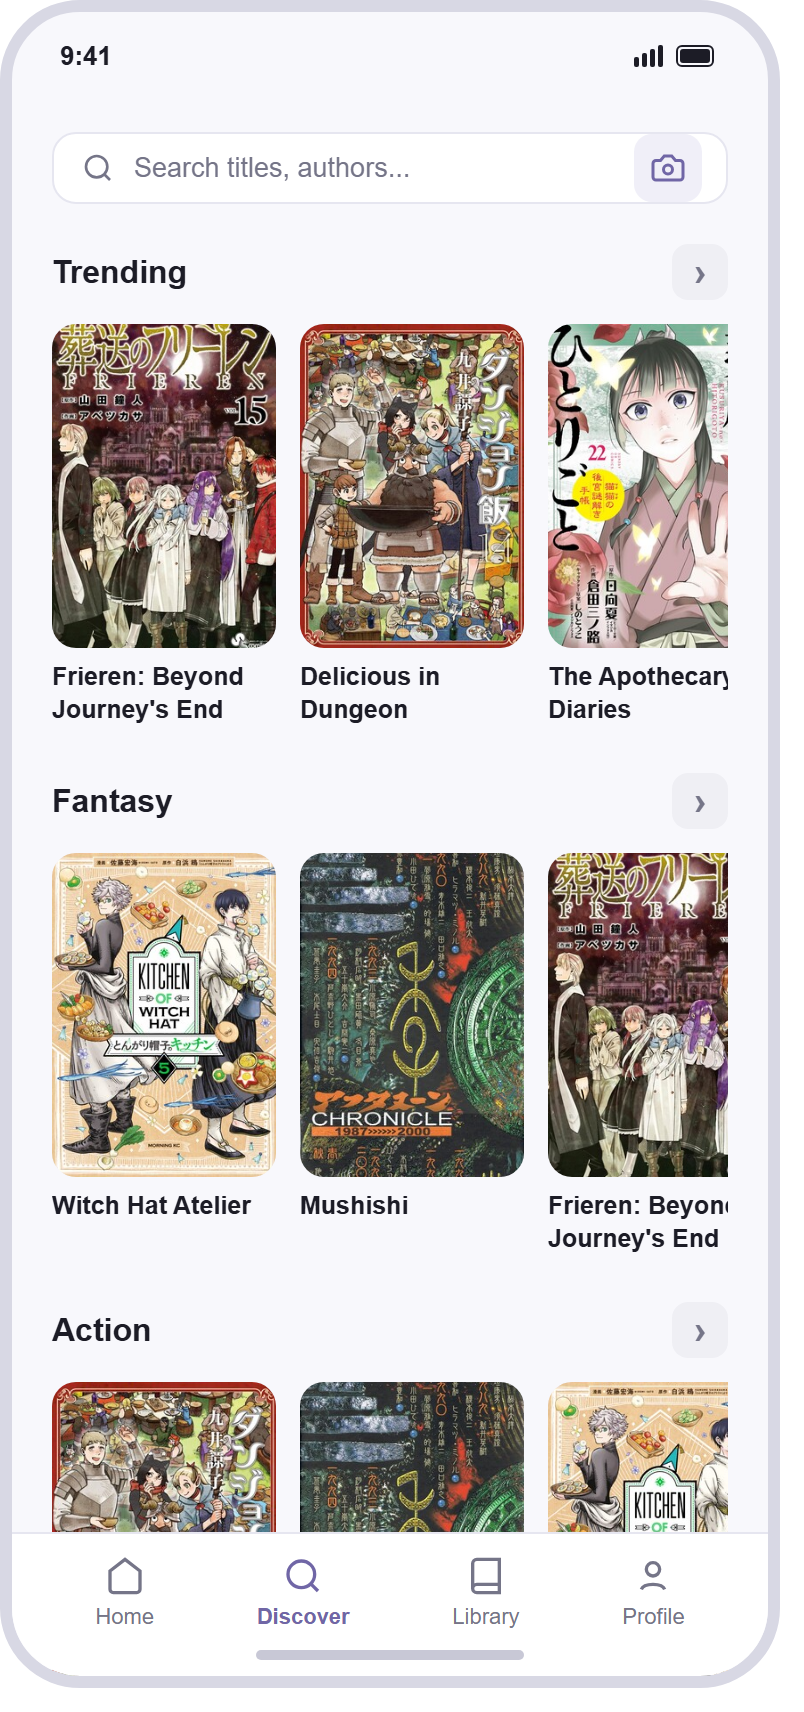
\includegraphics[width=\textwidth]{figures/ui/S03.png}
        \caption{\textbf{S03:} Discover}
    \end{subfigure}
    \hfill
    \begin{subfigure}[b]{0.24\textwidth}
        \centering
        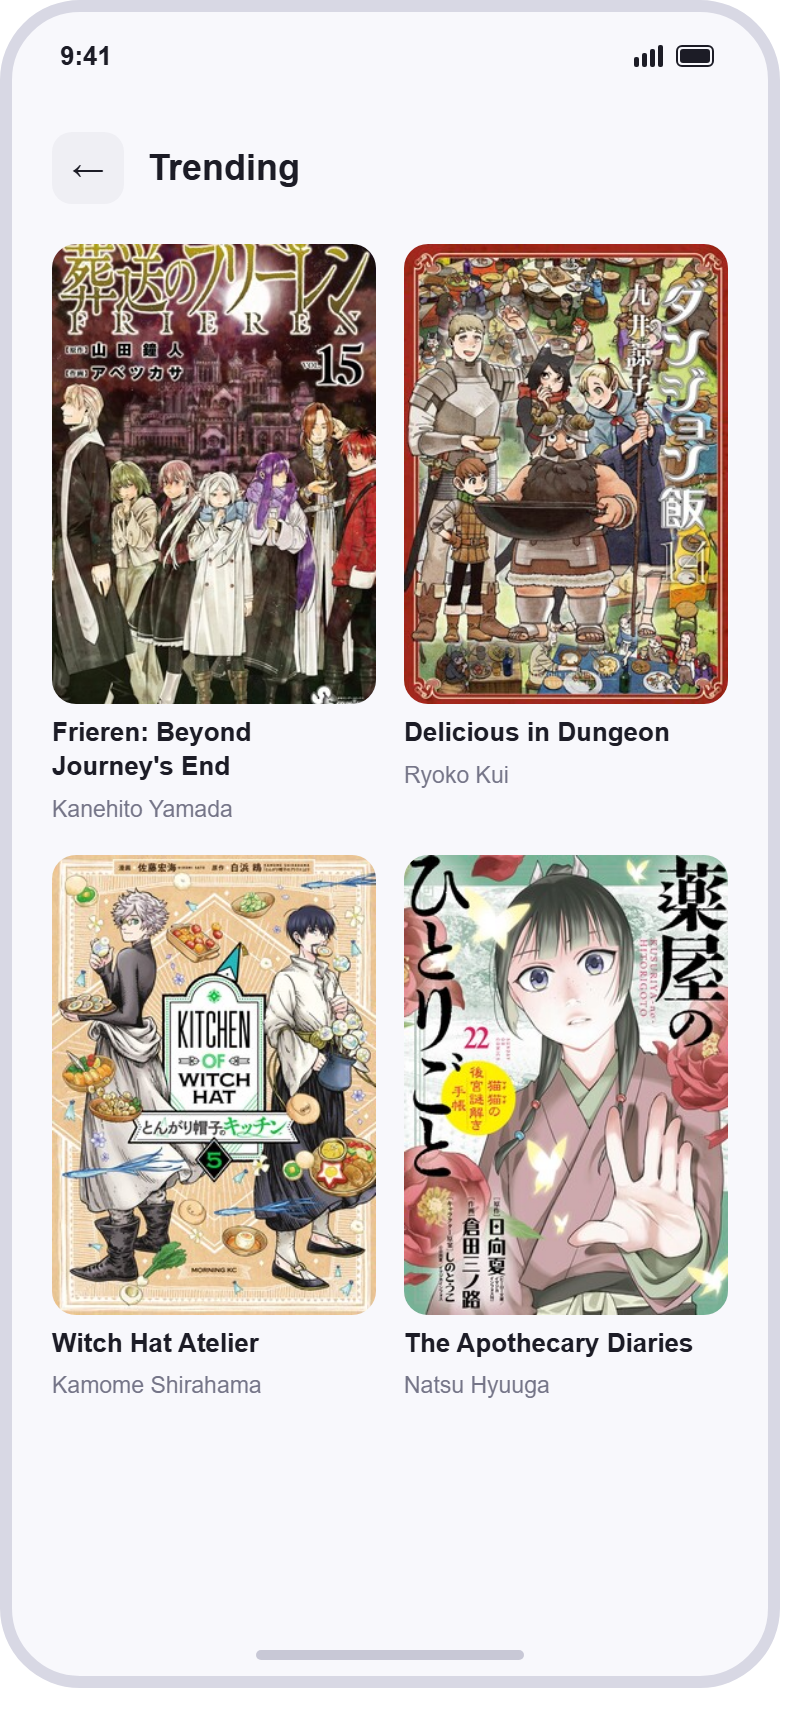
\includegraphics[width=\textwidth]{figures/ui/S03b.png}
        \caption{\textbf{S03b:} Expanded Grid}
    \end{subfigure}
    \caption{High-Fidelity Mockups (Part 1/3): Authentication (\texttt{S01}), 3-Block Home Feed (\texttt{S02}), Discover with AI Photo Search (\texttt{S03}), and Expanded Category Grid (\texttt{S03b}).}
    \label{fig:mockups_group1}
\end{figure}

\begin{figure}[H]
    \centering
    \begin{subfigure}[b]{0.24\textwidth}
        \centering
        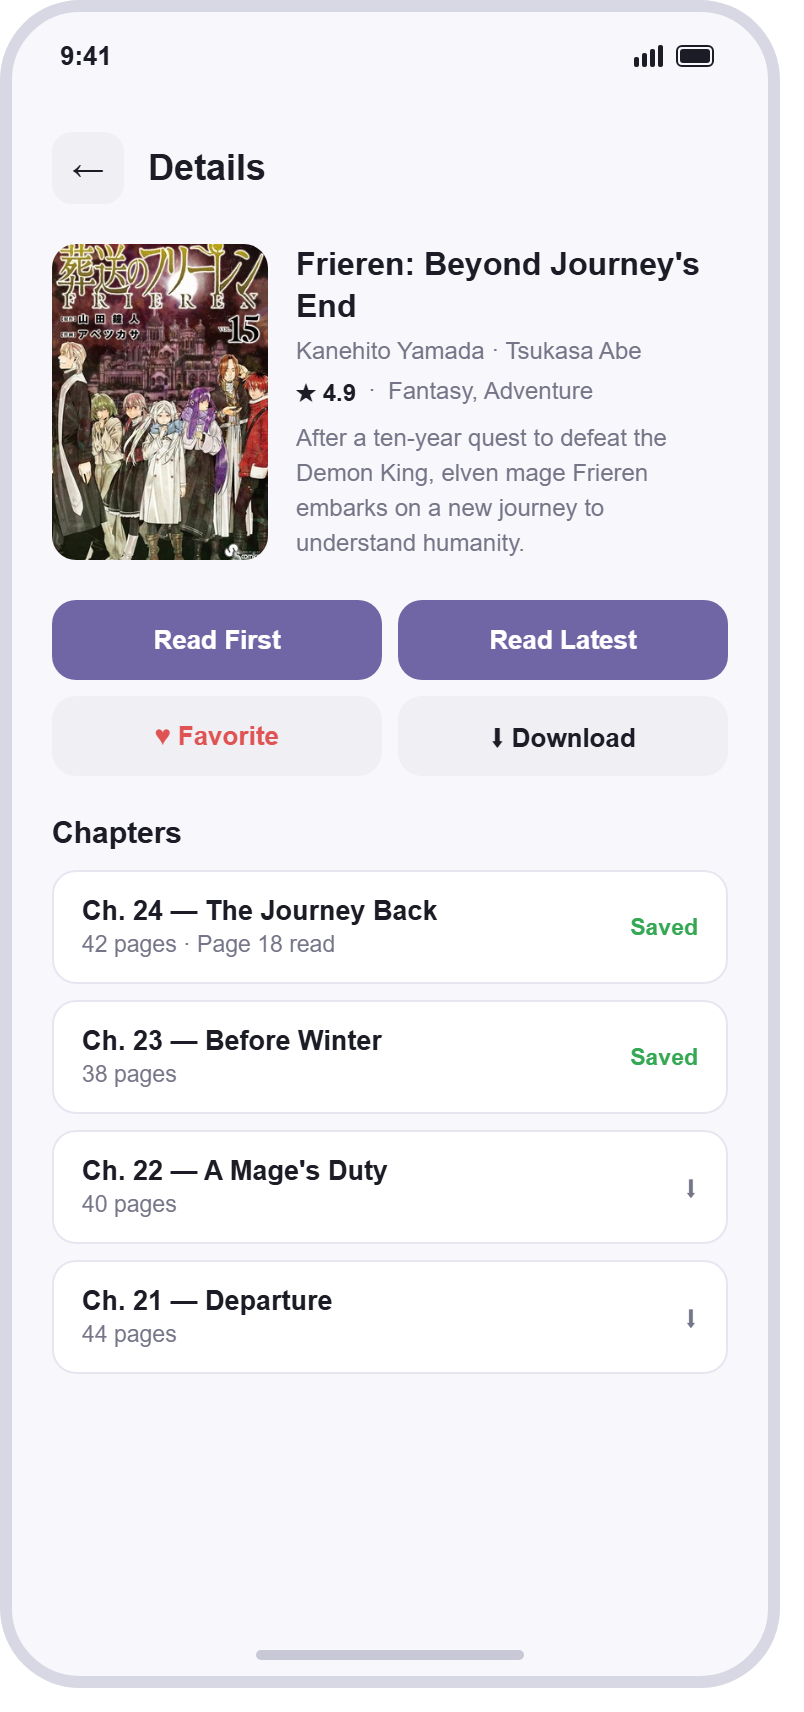
\includegraphics[width=\textwidth]{figures/ui/S04.png}
        \caption{\textbf{S04:} Manga Detail}
    \end{subfigure}
    \hfill
    \begin{subfigure}[b]{0.24\textwidth}
        \centering
        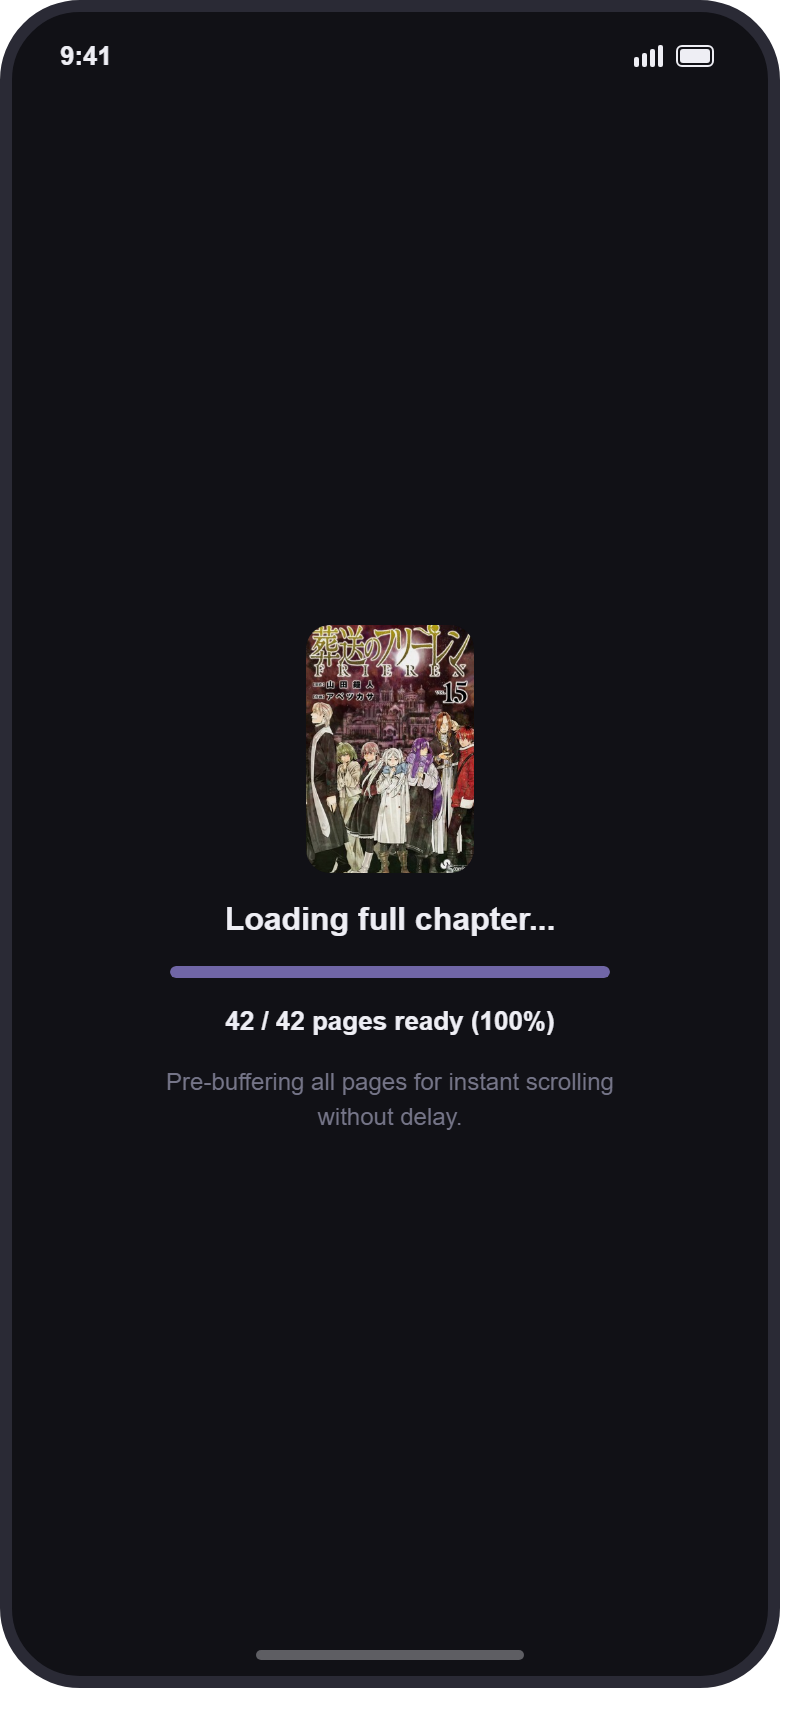
\includegraphics[width=\textwidth]{figures/ui/S10.png}
        \caption{\textbf{S10:} Chapter Preload}
    \end{subfigure}
    \hfill
    \begin{subfigure}[b]{0.24\textwidth}
        \centering
        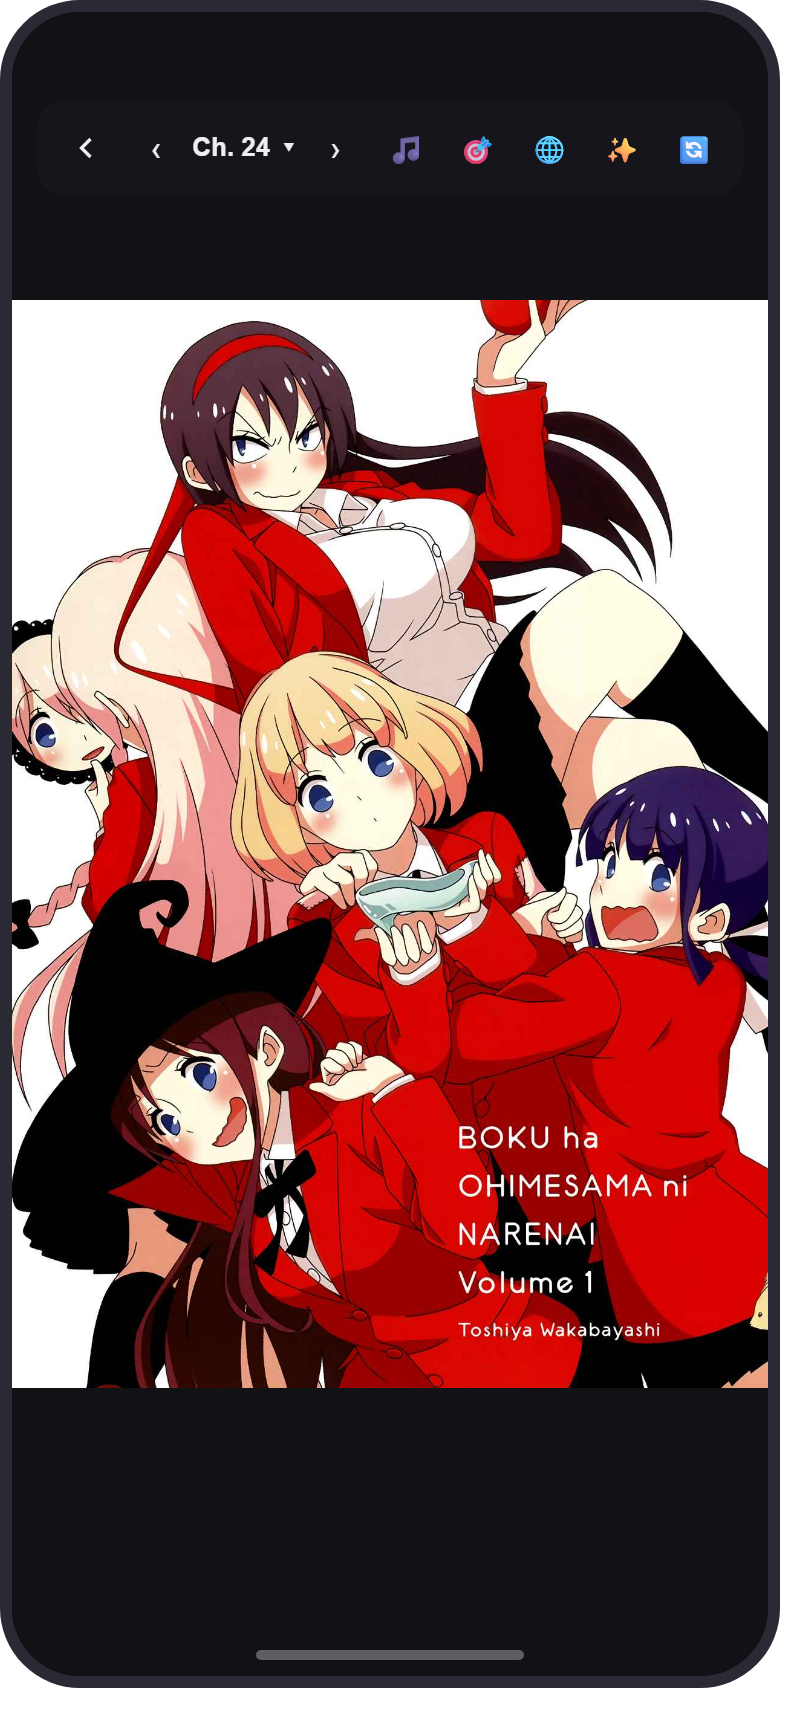
\includegraphics[width=\textwidth]{figures/ui/S05.png}
        \caption{\textbf{S05:} Full Reader}
    \end{subfigure}
    \hfill
    \begin{subfigure}[b]{0.24\textwidth}
        \centering
        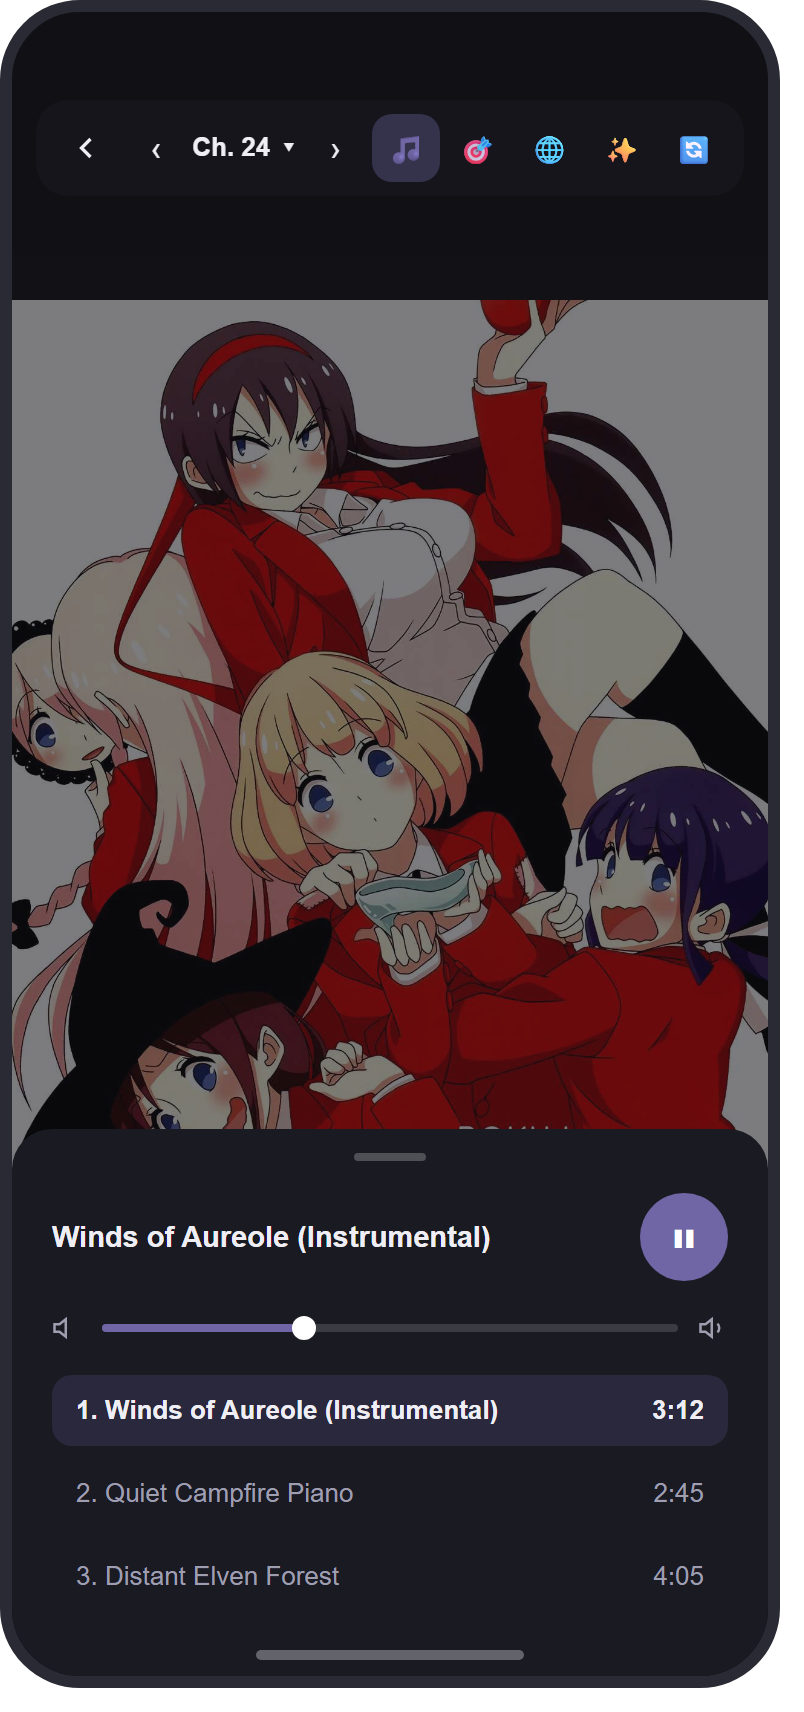
\includegraphics[width=\textwidth]{figures/ui/S06.png}
        \caption{\textbf{S06:} Audio Sheet}
    \end{subfigure}
    \caption{High-Fidelity Mockups (Part 2/3): Manga Detail (\texttt{S04}), Full-Chapter Preload State (\texttt{S10}), 100\% Full-Screen Reader (\texttt{S05}), and Genre Instrumental Audio Sheet (\texttt{S06}).}
    \label{fig:mockups_group2}
\end{figure}

\begin{figure}[H]
    \centering
    \begin{subfigure}[b]{0.24\textwidth}
        \centering
        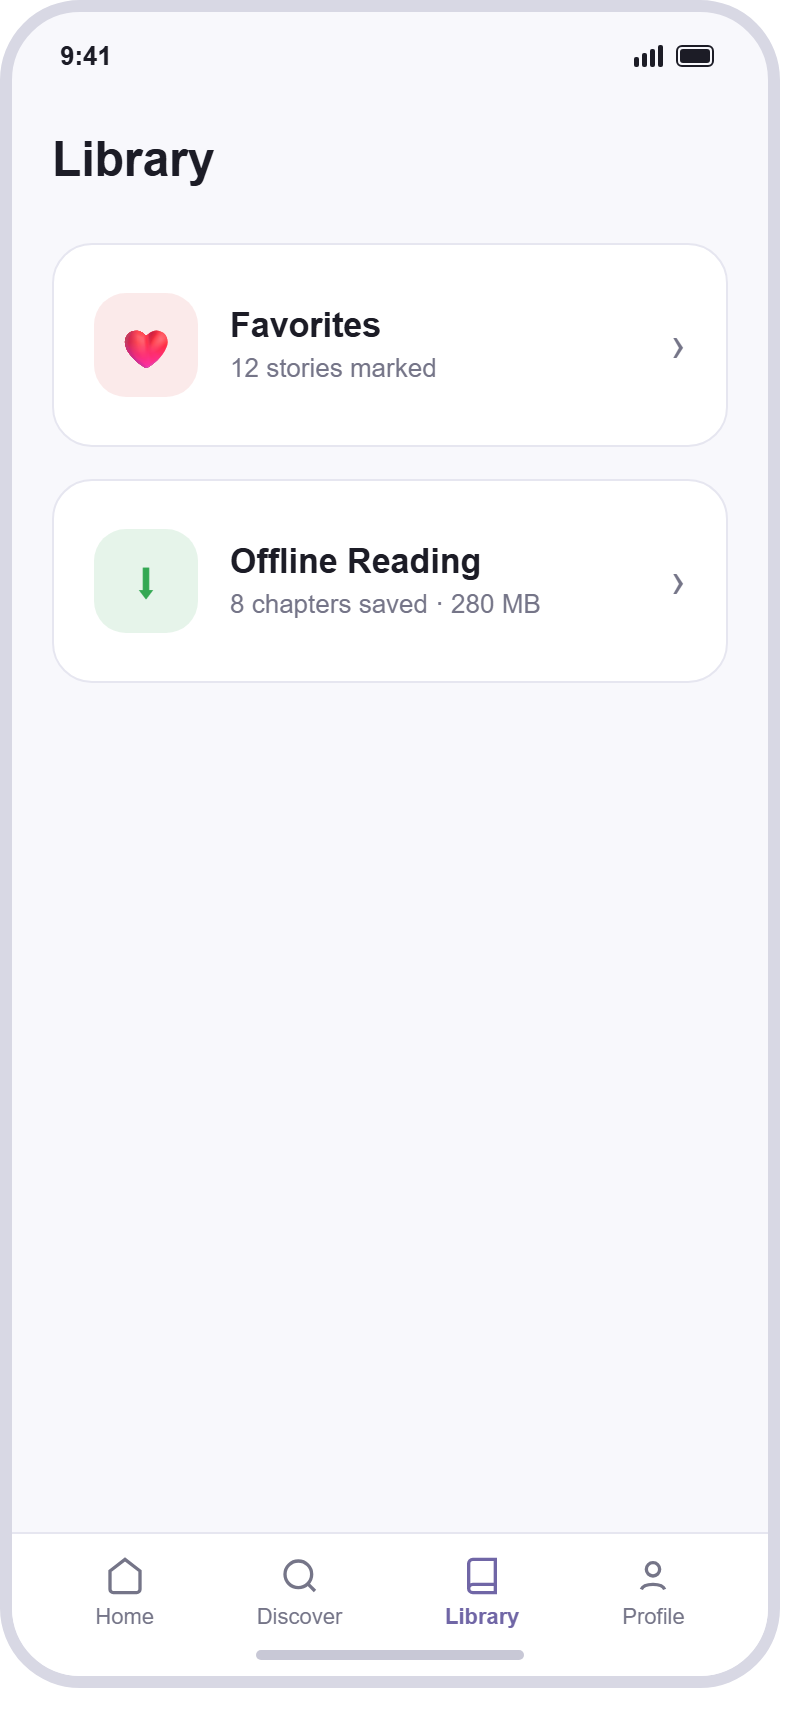
\includegraphics[width=\textwidth]{figures/ui/S07.png}
        \caption{\textbf{S07:} Library Hub}
    \end{subfigure}
    \hfill
    \begin{subfigure}[b]{0.24\textwidth}
        \centering
        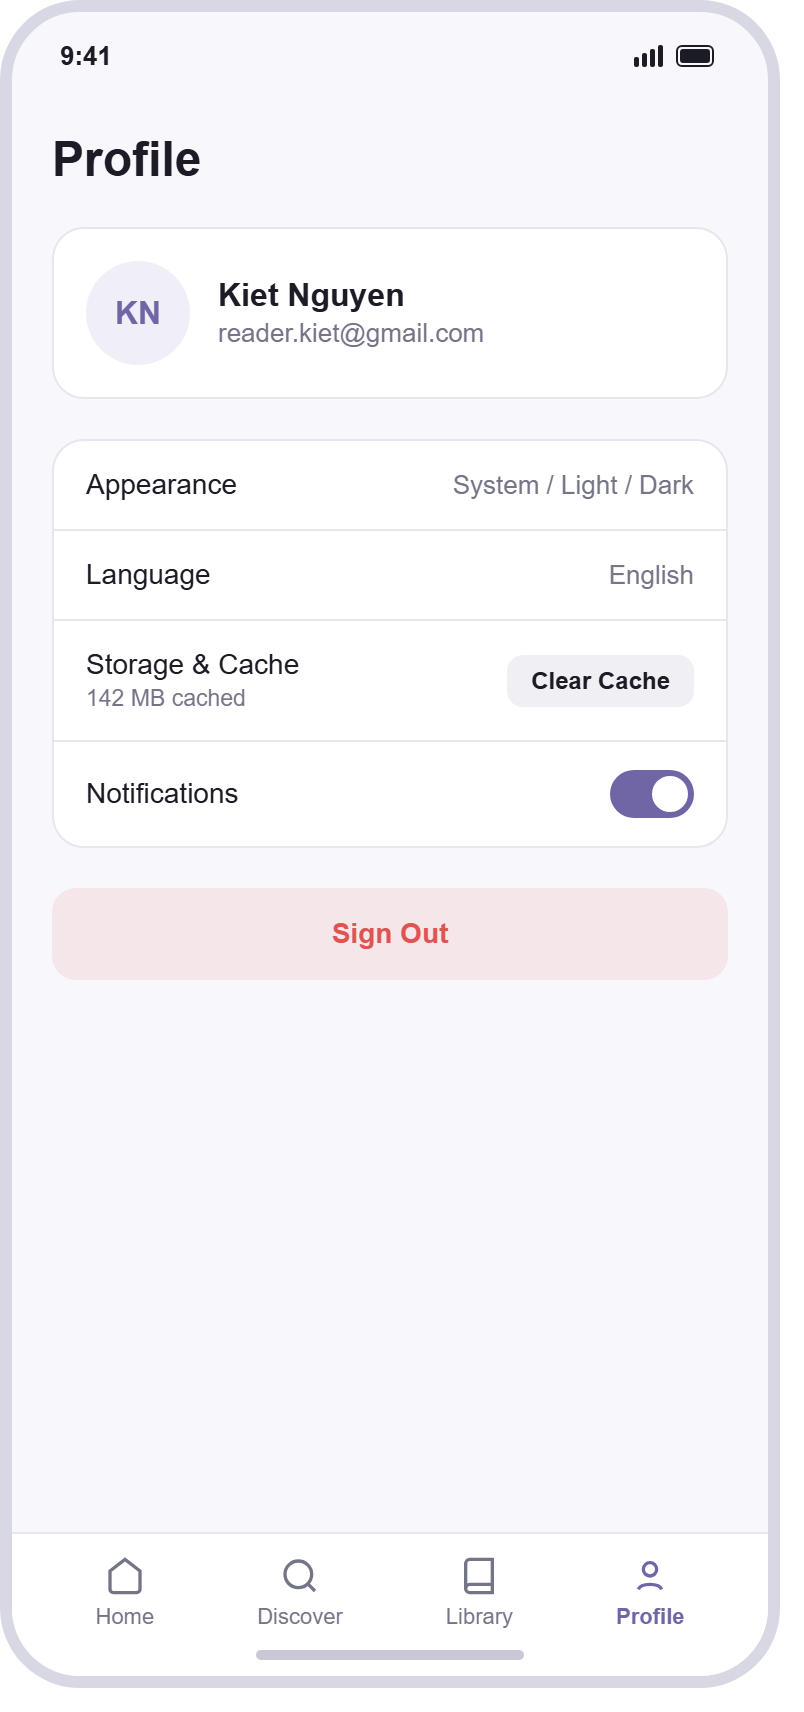
\includegraphics[width=\textwidth]{figures/ui/S08.png}
        \caption{\textbf{S08:} Profile \& Settings}
    \end{subfigure}
    \hfill
    \begin{subfigure}[b]{0.24\textwidth}
        \centering
        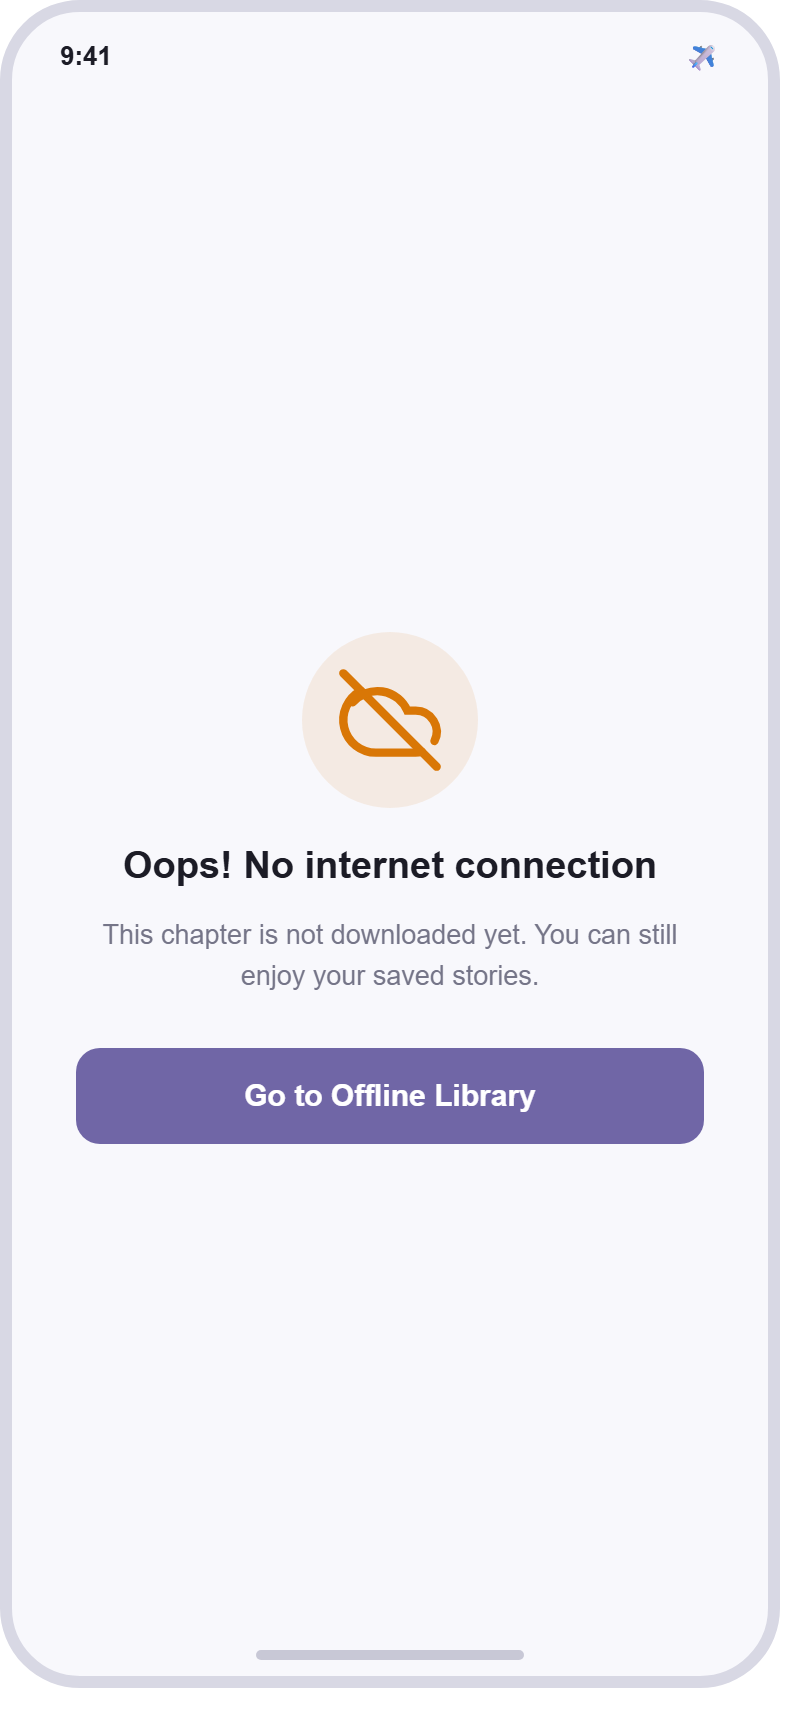
\includegraphics[width=\textwidth]{figures/ui/S09.png}
        \caption{\textbf{S09:} Offline Error}
    \end{subfigure}
    \hfill
    \begin{subfigure}[b]{0.24\textwidth}
        \centering
        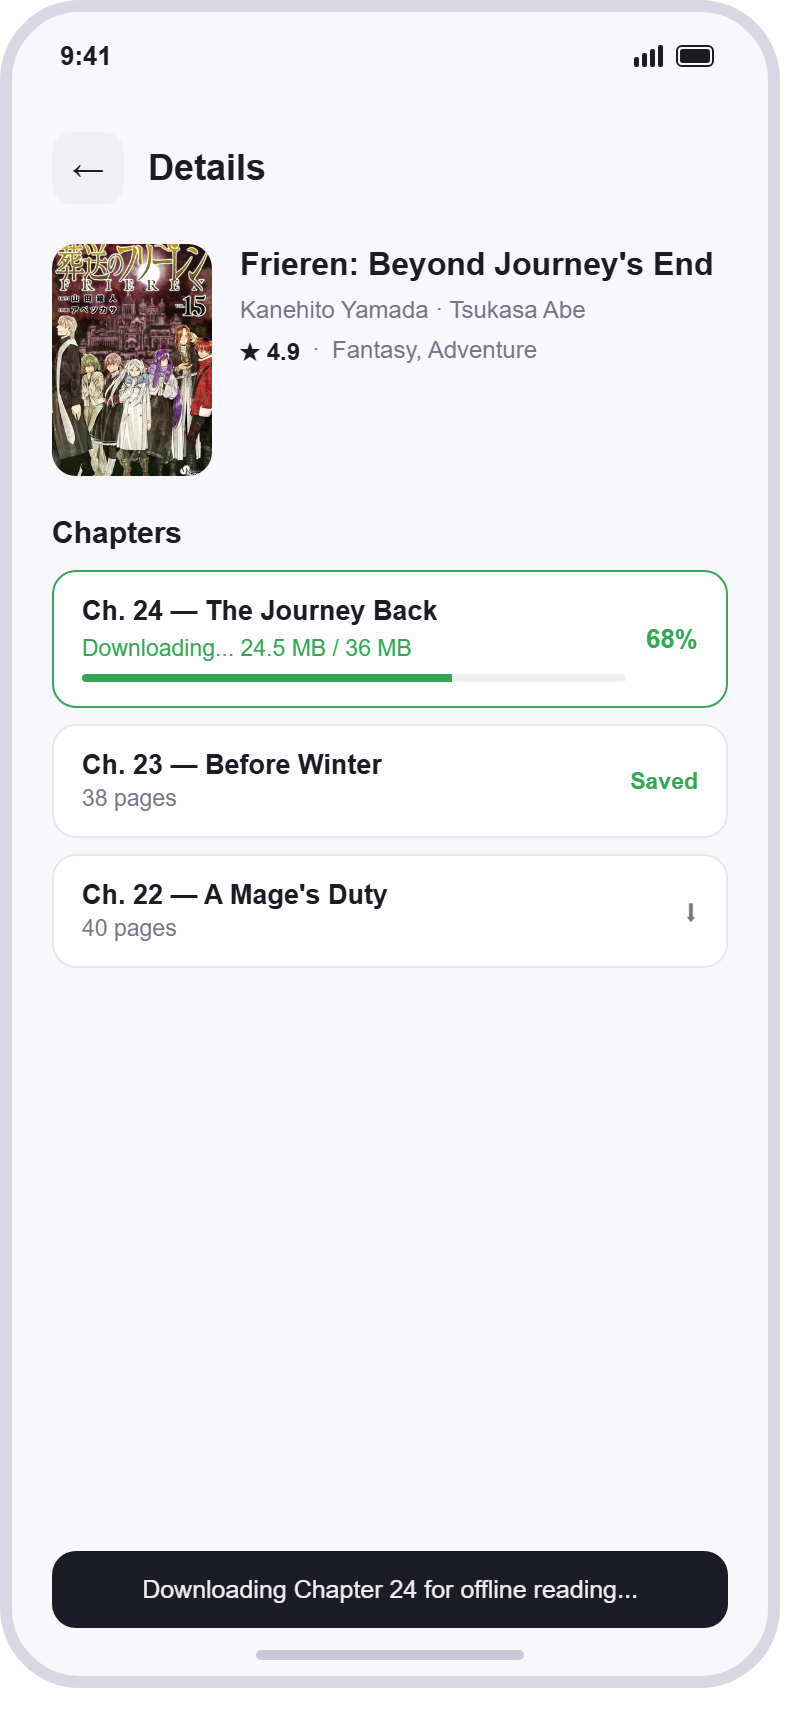
\includegraphics[width=\textwidth]{figures/ui/S11.png}
        \caption{\textbf{S11:} Download (68\%)}
    \end{subfigure}
    \caption{High-Fidelity Mockups (Part 3/3): Two-Button Library (\texttt{S07}), Profile \& Settings (\texttt{S08}), Offline Network Error State (\texttt{S09}), and Real-Time Download Progress State (\texttt{S11}).}
    \label{fig:mockups_group3}
\end{figure}

\begin{table}[H]
\centering
\caption{Comprehensive Specification of all 12 UI/UX Frames (\texttt{S01} to \texttt{S11}) including Primary, Loading, Error, and Offline States.}
\label{tab:screen_catalog}
\scriptsize
\renewcommand{\arraystretch}{1.24}
\begin{tabularx}{\textwidth}{C{1.1cm} L{2.8cm} C{2.1cm} Y}
\toprule
\rowcolor{tablehead}
\textbf{Frame} & \textbf{Screen Title} & \textbf{UI State Role} & \textbf{Key Components, Interactions \& Design Rules} \\
\midrule
\textbf{S01} & \textbf{Sign In} & Auth Entry & Bold lavender \textbf{NAOMI} wordmark (\texttt{\#7066A6}), Email \& Password inputs (\texttt{12px} radius), primary \textbf{Sign In} button, \textbf{Sign Up} and \textbf{Forgot Password?} links. Zero third-party social clutter. \\
\rowcolor{tablerow}
\textbf{S02} & \textbf{Home} & Primary Feed & Strictly 3 blocks: (1) Lavender-tinted \textbf{Continue Reading} Hero card (\textit{Frieren Ch.\ 24 $\cdot$ Page 18/42 (43\%)}) with 1-tap \textbf{Continue $\blacktriangleright$} pill; (2) \textbf{Recent} horizontal scroll; (3) \textbf{Recommended} horizontal scroll + 4-tab Bottom Nav. \\
\textbf{S03} & \textbf{Discover} & Search \& Browse & Search input (\textit{``Search titles, authors...''}) with trailing \textbf{Camera Icon} (invokes zero-permission OS Photo Picker for \texttt{FR-11}), followed by \textbf{Trending} and \textbf{Genre} (\textit{Fantasy, Action}) horizontal rows with \texttt{[>]} expand buttons. \\
\rowcolor{tablerow}
\textbf{S03b} & \textbf{Expanded List} & Category Grid & Full-screen 2-column vertical grid triggered by tapping \texttt{[>]} on \texttt{S03}; includes Back button (\texttt{$\leftarrow$}) and category header. \\
\textbf{S04} & \textbf{Manga Detail} & Series Hub & Cover artwork, title, author (\textit{Kanehito Yamada $\cdot$ Tsukasa Abe}), rating ($\star\ 4.9$), genres, synopsis, 4 action buttons (\textbf{Read First}, \textbf{Read Latest}, \textbf{$\heartsuit$ Favorite}, \textbf{$\downarrow$ Download}), and full chapter list with \textbf{Saved} badges. \\
\rowcolor{tablerow}
\textbf{S10} & \textbf{Full Chapter Preload} & \textbf{Loading State} & AMOLED dark screen (\texttt{\#111116}) with pulsing manga cover, \textit{``Loading full chapter... 42 / 42 pages ready (100\%)''} progress bar, pre-buffering all pages before opening \texttt{S05}. \\
\textbf{S05} & \textbf{Full Screen Reader} & Core Reader & $100\%$ full-screen manga artwork with a single translucent top bar: Back (\texttt{<}), Chapter switcher (\texttt{< Ch.\ 24 $\blacktriangledown$ >}), and 5 pure icons: Music ($\flat$), Focus Mode ($\odot$), Language ($\oplus$), AI Translate ($\star$), and Mode Toggle ($\leftrightarrows$). \\
\rowcolor{tablerow}
\textbf{S06} & \textbf{Audio Sheet} & Modal Overlay & Minimalist bottom sheet over \texttt{S05}: active genre instrumental title (\textit{Winds of Aureole}), $44\text{ px}$ Play/Pause button, smooth volume slider, and 3-row selectable track list for the active genre. \\
\textbf{S07} & \textbf{Library} & Collection Hub & Exactly \textbf{2 Large $20\text{ px}$-Radius Action Buttons}: (1) \textbf{$\heartsuit$ Favorites} (\textit{12 stories marked}) and (2) \textbf{$\downarrow$ Offline Reading} (\textit{8 chapters saved $\cdot$ 280 MB}). \\
\rowcolor{tablerow}
\textbf{S08} & \textbf{Profile \& Settings} & User \& System & Avatar (\texttt{KN}), \textit{Kiet Nguyen (reader.kiet@gmail.com)}, \textbf{Appearance} (\textit{System / Light / Dark}), \textbf{Language} (\textit{English / Tieng Viet}), \textbf{Storage \& Cache} (\textit{142 MB cached} + \textit{Clear Cache}), \textbf{Notifications}, and \textbf{Sign Out}. \\
\textbf{S09} & \textbf{Offline Error State} & \textbf{Error / Empty Fallback} & Triggered within $\le 300\text{ ms}$ when tapping an uncached chapter without Internet: amber offline cloud icon, \textit{``Oops! No internet connection''}, and primary CTA button \textbf{Go to Offline Library} $\to$ \texttt{S07}. \\
\rowcolor{tablerow}
\textbf{S11} & \textbf{Download in Progress} & \textbf{Active Progress State} & Highlights Chapter 24 row in sage green (\texttt{\#34A853}) with live progress bar (\textit{``Downloading... 24.5 MB / 36 MB -- 68\%''}) and bottom toast banner (\textit{``Downloading Chapter 24 for offline reading...''}). \\
\bottomrule
\end{tabularx}
\end{table}
